% !TeX root = orbits.tex

%%%%%%%%%%%%%%%%%%%%%%%%%%%%%%%%%%%%%%%%%%%%%%%%%%%%%%%%%%%%%%%%

\thispagestyle{empty}

\begin{center}
\textbf{\LARGE The Mathematics of Planetary Orbits}

\bigskip
\bigskip
\bigskip

\textbf{\Large Moti Ben-Ari}

\bigskip

\url{http://www.weizmann.ac.il/sci-tea/benari/}

\bigskip
\bigskip
\bigskip

Version $0.9$

\bigskip

\today

\end{center}

\vfill

\begin{center}
\copyright{} Moti Ben-Ari $2023$
\end{center}
 
\begin{small}
This work is licensed under Attribution-ShareAlike 4.0 International. To view a copy of this license, visit \url{http://creativecommons.org/licenses/by-sa/4.0/}.
\end{small}

\newpage

\tableofcontents

\newpage

\section{Introduction}

Everyone ``knows'' that Kepler discovered that the orbits of the planets are ellipses and that Newton showed that an elliptical orbit implies that the force of gravity must be inversely proportional to the square of the distance from the Sun. Although I knew these facts, I had never seen them demonstrated.

\textit{Calculus in Context} \cite{hahn-cic} by Alexander J. Hahn is a comprehensive textbook on introductory calculus that augments theory with  applications in physics and astronomy, such as the work of Kepler, Newton and Galileo, as well as applications in engineering such as building bridges and domed structures. These are not just historical anecdotes but detailed computations.

This document works out one topic based on the presentation in the book: the determination of orbits by Aristarchus, Copernicus, Kepler and Newton. The presentation is mathematical, since the historical and astronomical aspects are thoroughly described in \cite{hahn-cic}, as well as in other works. The document is intended to enrich the learning of mathematics by secondary-school students and students in introductory university courses.

Section~\ref{s.aristarchus} presents the measurements of the radii and distances of the Earth, the Moon and the Sun by Eratosthenes and Aristarchus. Section~\ref{s.copernicus} describes the construction of a model of a Sun-centered system by Copernicus. Section~\ref{s.kepler} shows how Kepler developed his three laws of planetary motion and Section~\ref{s.newton} presents Newton's derivation of the inverse-square law of gravitation from of Kepler's laws. One step of Newton's derivation requires a theorem whose proof is very long, so it is split off into Section~\ref{s.centripetal}. Appendix~\ref{s.ellipse} contains more than you ever wanted to know about the mathematics of ellipses, but these theorems are necessary. I suggest that you look up each theorem (and its proof) as needed, rather than trying to study them all at once.

The computations in Hahn's book are faithful to the historical record, for example, measuring distances in units such as the stadia of the Greeks. Here,  the computations are fully modernized and use modern units such as kilometers.

It is easy to measure angles. We are familiar with the use of a protractor\footnote{More precisely, a device for measuring angles is called a \emph{goniometer}.} in school and these can be scaled-up to obtain more accurate measurements. Measuring long distances was impossible until the recent inventions of radar and lasers. At most one could pace-off distances with low accuracy. The only \emph{measured} distance used here is the estimate of $800$ km by Eratosthenes for the distance between two places in Egypt (Section~\ref{s.eratosthenes}).

This documents uses many diagrams to facilitate understanding each step in the geometrical proofs, more than appear in other sources. For example, Newton proved his difficult theorem (Section~\ref{s.centripetal}) using only a single diagram. The diagrams are not to scale and are often distorted. Otherwise, it would be impossible to draw the Earth, Moon and Sun on a piece of paper, since the Sun is almost $400$ times farther away from the Earth than the Moon. If we drew the Moon one centimeter from the Earth, we would have to draw the Sun four meters away!

The prerequisites for reading the document are a good knowledge of Euclidean geometry, some trigonometry, a bit calculus and Newton's laws of motions. In particular you must know that if a sector of a circle subtends an angle of $\theta$ radians, the length of the sector is $r\theta$, where $r$ is the radius of the circle (Figure~\ref{f.radians}).

\begin{figure}[t]
\begin{center}
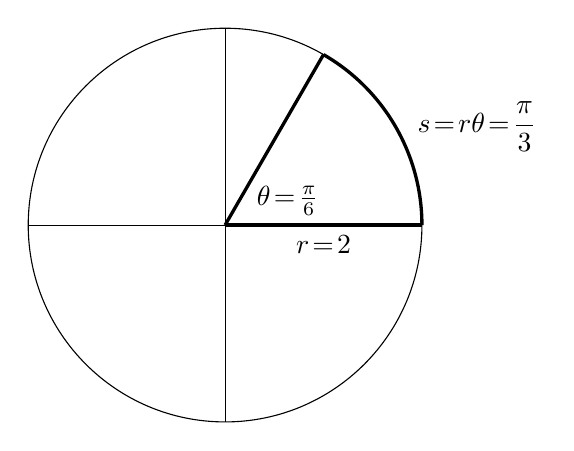
\begin{tikzpicture}
\node[draw,circle,minimum size=5cm] at (0,0) {};
\draw (-2.5,0) -- (2.5,0);
\draw (0,-2.5) -- (0,2.5);
\draw[very thick] (0,0) -- node[below] {$r\!=\!2$} (2.5,0);
\draw[very thick] (0,0) -- (60:2.5);
\node[above right,xshift=8pt] at (0,0) 
  {$\theta\!=\!\frac{\pi}{6}$};
\draw[very thick] (2.5,0) arc(0:60:2.5)
  node[right,midway,xshift=4pt]
    {$s\!=\!r\theta\!=\!\displaystyle\frac{\pi}{3}$};
\end{tikzpicture}
\caption{Angles and arcs}\label{f.radians}
\end{center}
\end{figure}

\subsection*{Notation}

The following shortcuts facilitate a less verbose presentation:
\begin{itemize}
\item $a$ and $b$ denote the semi-major and semi-minor axes of an ellipse.
\item $AB$ denotes both a line segment and its length.
\item $\triangle ABC$ denotes both a triangle and its area.
\item The diagram below shows that when the line segment $AB$ is \emph{extended} it intersects the line $CD$ at a point $E$. The rather archaic term for extended is \emph{produced}. When the text says that $AB$ intersects $CD$, the intention is that $AB$ can produced or extended until it intersects $CD$.
\end{itemize}

\begin{center}
\begin{tikzpicture}
\draw (0,0) coordinate (A) node[below] {$A$} -- (2,0) coordinate(B) node[below] {$B$};
\draw (4.5,-.5) coordinate (C) node[below] {$C$} -- (5.5,.5) coordinate (D) node[above] {$D$}; 
\draw[dotted,thick] (B) -- (5,0) coordinate (E) node[xshift=6pt,right] {$E$};
%\vertexsm{A};
%\vertexsm{B};
%\vertexsm{C};
%\vertexsm{D};
\vertexsm{E};
\end{tikzpicture}
\end{center}

\subsection*{Acknowledgments}

I am grateful to Alex Hahn and Graham Griffiths for their guidance.
